\documentclass{article}

\usepackage{color}
\usepackage[top=1in,bottom=1in,left=1.2in,right=1.2in]{geometry}
\usepackage{hyperref}
\usepackage[small]{titlesec}
\usepackage{booktabs}
\usepackage{colm2024_conference}
\usepackage{graphicx}
\usepackage[dvipsnames]{xcolor}
\usepackage{rotating}
\usepackage{pdflscape}
\usepackage{amsmath}

\newcommand{\todo}[1]{\textcolor{red}{\textbf{TODO:} #1}}

% Commenting
\newcommand{\eat}[1]{\ignorespaces}
%% Comment this line and uncomment the next to hide all comments
\newcommand{\xxcomment}[4]{\textcolor{#1}{[$^{\textsc{#2}}_{\textsc{#3}}$ #4]}}
%\newcommand{\xxcomment}[4]{\eat{#1}}
\newcommand{\ya}[1]{\xxcomment{red}{Y}{A}{#1}}
\newcommand{\ta}[1]{\xxcomment{blue}{T}{A}{#1}}


\title{CSE 5525: Assignment 3}

\author{Kurt Wanner}

\date{}


\colmfinalcopy
\begin{document}
\maketitle


\section{Data Statistics and Processing (8pt)}
\paragraph{Instructions:} Use \autoref{tab:data_stats_before} and \autoref{tab:data_stats_after} to describe the data statistics before and after any pre-processing respectively. 
Use the T5 tokenizer to report the statistics. 
For the statistics after pre-processing, if you did different pre-processing for different models, you need to indicate them separately.
The gray text in each row is there to guide you and should be removed in your submitted report.
Depending on your pre-processing, some numbers may be identical across tables. 

\begin{table}[h!]
\centering
\begin{tabular}{lcc}
\toprule
Statistics Name & Train & Dev \\
\midrule
Number of examples & \textcolor{gray}{4225} & \textcolor{gray}{466} \\
Mean sentence length & \textcolor{gray}{18.10}& \textcolor{gray}{18.07} \\
Mean SQL query length & \textcolor{gray}{218.37}& \textcolor{gray}{212.05}  \\
Vocabulary size (natural language)& \textcolor{gray}{792}& \textcolor{gray}{466}  \\
Vocabulary size (SQL)& \textcolor{gray}{557}& \textcolor{gray}{397}  \\
\bottomrule
\end{tabular}
\caption{Data statistics before any pre-processing. \textcolor{gray}{You need to at least provide the statistics listed above, and can add new entries.}}
\label{tab:data_stats_before}
\end{table}

\begin{table}[h!]
\centering
\begin{tabular}{lcc}
\toprule
Statistics Name & Train & Dev \\
\midrule
\multicolumn{3}{l}{\textbf{Model: T5 Fine-tuning \& T5 from Scratch}} \\ % \textcolor{gray}{(T5 fine-tuning or T5 from scratch)}} \\
Mean sentence length & \textcolor{gray}{8.43}& \textcolor{gray}{8.35} \\
Mean SQL query length & \textcolor{gray}{126.14}& \textcolor{gray}{121.96} \\
Vocab size (NL) & \textcolor{gray}{727}& \textcolor{gray}{379} \\
Vocab size (SQL) & \textcolor{gray}{491}& \textcolor{gray}{299} \\
\bottomrule
\end{tabular}
\caption{Data statistics after pre-processing. \textcolor{gray}{You need to at least provide the statistics listed in \autoref{tab:data_stats_before} (except for the number of lines), and can add new entries.}}
\label{tab:data_stats_after}
\end{table}



\newpage




\section{T5 Fine-tuning and Training From Scratch (8pt)}\label{sec:t5}
\paragraph{Instructions:} Use \autoref{tab:t5_results_ft} and \autoref{tab:t5_results_scratch} to describe your data processing steps (if any) and the implementation details, respectively for the fine-tuned T5 model, and the T5 model trained from scratch.
The gray text in each row is there to guide you and should be removed in the submitted report. 
Be clear enough that we can replicate your approach in PyTorch using only your descriptions.

\begin{table}[h!]
\centering
\begin{tabular}{p{3.5cm}p{10cm}}
\toprule
Design choice & Description \\
\midrule
Data processing & The first step was to remove stop words. This list can be found in  \verb|data/stop_words.txt| and \verb|data/stop_phrases.txt|. Next, proper names (i.e. houston, california, atlanta airport, etc.) were converted to their SQL counterparts (i.e. 'HOUSTON', 'CALIFORNIA', and 'ATL').  \\
Tokenization & The default T5 tokenizer was used with additional added tokens. These additional tokens can be found in \verb|data/tokens_nl.txt| and \verb|data/tokens_sql.txt|. \\
Architecture & Because of the additional tokens, I resized the token embeddings. For fine-tuning, the entire model was tuned. To increase training speed, the model's parameters were converted to type bfloat16. \\
Hyperparameters & 
\textbf{Learning Rate:} \textcolor{gray}{3e-5}
 
\textbf{Batch Size:} \textcolor{gray}{16} 

\textbf{Stopping Criteria:} \textcolor{gray}{Training periods of 15 epochs each, repeated until improvements in Record F1 slowed.} 

\textbf{LR Scheduler:} \textcolor{gray}{Cosine}  \\
\bottomrule
\end{tabular}
\caption{Details of the best-performing T5 model configurations (fine-tuned)}
\label{tab:t5_results_ft}
\end{table}


\begin{table}[h!]
\centering
\begin{tabular}{p{3.5cm}p{10cm}}
\toprule
Design choice & Description \\
\midrule
Data processing & The Data Processing was identical to the fine-tuned model. \\
Tokenization & The tokenization was identical to the fine-tuned model. \\
Architecture & Similar to the fine-tuned model, the model's parameters were converted to type bfloat16 to improve training speed. \\
Hyperparameters & \textbf{Learning Rate:} \textcolor{gray}{1e-4}

\textbf{Batch Size:} \textcolor{gray}{8} 

\textbf{Stopping Criteria:} \textcolor{gray}{Training periods of 15 epochs each, repeated until improvements in Record F1 slowed.} 

\textbf{LR Scheduler:} \textcolor{gray}{Cosine}  \\
\bottomrule
\end{tabular}
\caption{Details of the best-performing T5 model configurations (from scratch)}
\label{tab:t5_results_scratch}
\end{table}


\newpage



\section{Large Language Model (LLM) Prompting (14pt)}\label{sec:llm}

\subsection{In-Context Learning (ICL)}\label{sec:llm:icl}

\paragraph{Instructions:} Provide in \autoref{tab:icl_prompts} the instruction prompt(s) that you used for ICL.

If the prompt you used for zero- and few-shot prompting is identical, except for the examples, there's no need to repeat it. 
If you made small modifications between zero- and few-shot, please provide them separately.
For all entries, you need to specify the corresponding values of $k$.




\begin{table}[h!]
\centering
\begin{tabular}{p{1cm}p{12cm}}
\toprule
\textbf{Shot} & \textbf{Prompt} \\
\midrule
    \textcolor{gray}{0} & \textcolor{gray}{You are a very powerful text-to-sql model.} \\
    & \textcolor{gray}{Given the following SQL tables, create an SQL query for a user request.} \\
	& \textcolor{gray}{} \\
	& \textcolor{gray}{[SCHEMA FOR FLIGHT DATABASE]} \\
	& \textcolor{gray}{} \\
	& \textcolor{gray}{Create an SQL Query for the following question.} \\
	& \textcolor{gray}{Only return the output and nothing else.} \\
	& \textcolor{gray}{[Question]: [NL INSTRUCTION]} \\
	& \textcolor{gray}{[Answer]: } \\
\midrule
	\textcolor{gray}{$k > 0$} & \textcolor{gray}{You are a very powerful text-to-sql model. }\\
	& \textcolor{gray}{Given the following SQL tables, create an SQL query for a user request.} \\
	& \textcolor{gray}{} \\
	& \textcolor{gray}{[SCHEMA FOR FLIGHT DATABASE]} \\
	& \textcolor{gray}{} \\
	& \textcolor{gray}{[Question]: [TRAINING NL INSTRUCTION] }\\
	& \textcolor{gray}{[Answer]: [CORRESPONDING SQL QUERY]} \\
	& \\
	& \textcolor{gray}{\vdots} \\
	& \\
	& \textcolor{gray}{Base your answer on these examples.} \\
	& \textcolor{gray}{Create an SQL Query for the following question.} \\
	& \textcolor{gray}{Only return the output and nothing else.} \\
	& \textcolor{gray}{[Question]: [NL INSTRUCTION]} \\
	& \textcolor{gray}{[Answer]: } \\
\bottomrule
\end{tabular}
\caption{Instruction prompts used for zero- and/or few-shot prompting.}
\label{tab:icl_prompts}
\end{table}

\paragraph{Example selections:} Please provide a clear, detailed, and succinct description of how you selected the examples when $k > 0$.

\textcolor{gray}{The examples were chosen dynamically based on a simple similarity score between the given NL instruction and all training examples. The similarity score is based on the set of key words in each NL instruction. This list of key words can be found in} \verb|data/prompt_key_words.txt|.

\textcolor{gray}{The calculation for the similarity score is $Score(key_1, key_2) = |key_1$ \textbackslash  $ key_2| + |key_2$ \textbackslash  $ key_1|$}
 
\newpage


\subsection{Best Prompt and Ablation Study}

\paragraph{Instructions:} Report the best prompt you used in \autoref{tab:best_prompt}.
If the best prompt you used is the same as the one specified in \autoref{tab:icl_prompts}, you can just copy the best prompt and label it.
If it is different (e.g. you designed another prompt that is better), you should clearly describe how you created it and what are the methods you used in the caption.

You will also need to clearly and succintly describe in \autoref{tab:ablation_explanation} the ablation experiments that you performed by removing different parts of the prompt.
For that, you need to first highlight the parts of the prompt that you ablated for each experiment in a distinct color\footnote{\url{https://www.overleaf.com/learn/latex/Using_colors_in_LaTeX}}, as shows the placeholder example in \autoref{tab:icl_prompts}, and second, provide the description by referring to the highlighted part.
When reporting your results in \autoref{tab:results}, you will need to refer to your ablations variants.



\begin{table}[h!]
\centering
\begin{tabular}{p{13.5cm}}
\toprule
\textbf{Prompt} \\
\midrule
\textcolor{gray}{You are a very powerful text-to-sql model. }\\
\textcolor{gray}{Given the following SQL tables, create an SQL query for a user request.} \\
\textcolor{gray}{} \\
\textcolor{gray}{[SCHEMA FOR FLIGHT DATABASE]} \\
\textcolor{gray}{} \\
\textcolor{gray}{[Question]: [TRAINING NL INSTRUCTION] }\\
\textcolor{gray}{[Answer]: [CORRESPONDING SQL QUERY]} \\
\\
\textcolor{gray}{\vdots} \\
\\
\textcolor{gray}{Base your answer on these examples.} \\
\textcolor{gray}{Create an SQL Query for the following question.} \\
\textcolor{gray}{Only return the output and nothing else.} \\
\textcolor{gray}{[Question]: [NL INSTRUCTION]} \\
\textcolor{gray}{[Answer]: } \\
\bottomrule
\end{tabular}
\caption{The best prompt.
{\textcolor{gray}{My best prompt was the prompt from \autoref{tab:icl_prompts}}}
}
\label{tab:best_prompt}
\end{table}



\begin{table}[h!]
\centering
\begin{tabular}{p{2cm}p{10cm}}
\toprule
\textbf{Color} & \textbf{Description} \\
\midrule
\textcolor{Red}{Red} & \textcolor{Red}{In this experiment, the Red text was removed.} \\
\textcolor{Blue}{Blue} & \textcolor{Blue}{In this experiment, the Blue text was removed.} \\
\textcolor{Purple}{Purple} & \textcolor{Purple}{In this experiment, both the Red and Blue text was removed.} \\
% \midrule
\bottomrule
\end{tabular}
\caption{Ablation variants.
{\textcolor{gray}{Put a clear description of the ablation experiments you did. If it helps to describe more clearly, you can also provide an example of the relevant part of the prompt before and after the ablation.}
}}
\label{tab:ablation_explanation}
\end{table}



\newpage



\section{Results and Analysis (20pt)}

\paragraph{Quantitative Results:} Use \autoref{tab:results} to report your test and development set results. 
Your test results should match with the results on gradescope. 
For the development set, you should also report results from experiments you conducted to arrive at your final configuration.
When reporting experiments, you should replace "variant" with brief and meaningful descriptions of whatever hyperparameter or setting that you varied. 
For ICL, you should specify what is the parameter $k$ used, and what the full model corresponds to. For T5, the full model refers to the best model you described in Section \ref{sec:t5}.
For T5, if you experimented with different design choices, you can add rows specifying the variants and what you tried.
The text in gray is only for example purpose, and should be removed and replaced with your own choices.
You may add more rows if needed.

\begin{table}[h!]
\centering
\begin{tabular}{lcc}
  \toprule
  System & Query EM \% & F1 score\\
  \midrule
  \multicolumn{3}{l}{\textbf{Dev Results}} \\
  \midrule
  \multicolumn{3}{l}{\textbf{LLM Prompting}} \\
	Full Model: Gemma-2B &  &  \\ 
	ICL, $k=0$ & 0.0 & 11.80 \\
	ICL, $k=1$ & 0.0 & 11.25 \\
	ICL, $k=2$ & 0.0 & 11.76 \\
	ICL, $k=3$ & 0.0 & 12.33 \\
	\textcolor{Red}{Red Ablation}, $k=5$ & 1.5 & 15.66 \\
	\textcolor{Blue}{Blue Ablation}, $k=1$ & 0.0 & 11.77 \\
	\textcolor{Purple}{Purple Ablation}, $k=0$ & 0.0 & 11.80 \\
	\textcolor{Purple}{Purple Ablation}, $k=1$ & 0.0 & 12.42 \\
	\textcolor{Purple}{Purple Ablation}, $k=3$ & 0.0 & 12.08 \\
	
  \multicolumn{3}{l}{\textbf{T5 fine-tuned}} \\
  Full model & 4.94 & 87.90 \\[5pt]
  % Variant1 & XX.XX & XX.XX \\

  \multicolumn{3}{l}{\textbf{T5 from scratch}} \\
  Full model & 4.51 & 70.59 \\ 
  % Variant1 & XX.XX & XX.XX \\

  \midrule
  \multicolumn{3}{l}{\textbf{Test Results}} \\
  \midrule
  ICL & XX.XX & XX.XX \\ 
  T5 fine-tuning & XX.XX & XX.XX \\
  T5 from scratch & XX.XX & XX.XX \\
  \bottomrule
\end{tabular}  
\caption{Development and test results. \textcolor{gray}{Use this table to report quantitative results for both dev and test results, for all the three models.}}
\label{tab:results}
\end{table}


\paragraph{ICL sensitivity to $k$:} For ICL, please provide a plot of the Record F1 on the development set that the model achieved with different values of $k$. The x-axis should be $k$, and the y-axis the Record F1. The prompts and examples used for this plot should correspond to the ones you described in Subsection \ref{sec:llm:icl}.

\begin{center}
	\centering
	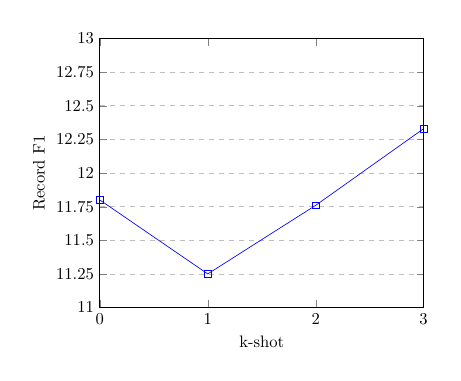
\begin{tikzpicture}[scale=0.6]
		\begin{axis}[
			xlabel={k-shot},
			ylabel={Record F1},
			xmin=0, xmax=3,
			ymin=11, ymax=13,
			xtick={0,1,2,3},
			ytick={11, 11.25, 11.5, 11.75, 12, 12.25, 12.5, 12.75, 13},
			legend pos=north west,
			ymajorgrids=true,
			grid style=dashed,
			]
			
			\addplot[
			color=blue,
			mark=square,
			]
			coordinates {
				(0,11.8)(1, 11.25)(2, 11.76)(3, 12.33)
			};
			
			
		\end{axis}
	\end{tikzpicture}
\end{center}


\newpage

\paragraph{Qualitative Error Analysis:} Conduct a detailed error analysis for each of the three models. Identify common error types and discuss possible reasons for these errors in \autoref{tab:qualitative}.

You must identify at least three classes of errors for the queries, and use examples to illustrate them.
It must be clear what model makes the errors you are analyzing. 
If you identified the same type of error for different models, you don't need to duplicate the descriptions, but you need to clearly specify an example for each of the model, indicate the statistics for each model, and specify to which model each statistics correspond to.
You may add more rows to the table.


\begin{landscape}
\begin{table}
  \centering
  \begin{tabular}{p{2cm}p{2cm}p{6cm}p{6cm}p{6cm}}
    \toprule
    \textbf{Error Type} & \textbf{Relevant Models}& \textbf{Example Of Error} & \textbf{Error Description} & \textbf{Statistics} \\
    \midrule
    \textcolor{gray}{Error name} & \textcolor{gray}{ICL, T5 fine-tuned or T5 from scratch} & \textcolor{gray}{Snippet from datapoint examplifying error} & \textcolor{gray}{Describe the error in natural language} & \textcolor{gray}{Provide statistics in the form ``COUNT/TOTAL'' on the prevalence of the error. TOTAL is the number of relevant examples (e.g. number of queries, for query-level error), and COUNT is the number of examples that showed this error.}  \\
    & & & & \textcolor{gray}{If an error type applies to several models, you should provide the statistics in the form ``MODEL NAME: COUNT/TOTAL''.} \\
    \midrule
    &  &  &  & \\
    \bottomrule
  \end{tabular}
  \label{tab:qualitative}
  \caption{Use this table for your qualitative analysis on the dev set, for all the three models.}\label{tab:qualitative}
\end{table}
\end{landscape}



\end{document}